% -*- mode: Latex; fill-column: 120; -*-
\documentclass{article}\usepackage[]{graphicx}\usepackage[]{color}
%% maxwidth is the original width if it is less than linewidth
%% otherwise use linewidth (to make sure the graphics do not exceed the margin)
\makeatletter
\def\maxwidth{ %
  \ifdim\Gin@nat@width>\linewidth
    \linewidth
  \else
    \Gin@nat@width
  \fi
}
\makeatother

\definecolor{fgcolor}{rgb}{0.345, 0.345, 0.345}
\newcommand{\hlnum}[1]{\textcolor[rgb]{0.686,0.059,0.569}{#1}}%
\newcommand{\hlstr}[1]{\textcolor[rgb]{0.192,0.494,0.8}{#1}}%
\newcommand{\hlcom}[1]{\textcolor[rgb]{0.678,0.584,0.686}{\textit{#1}}}%
\newcommand{\hlopt}[1]{\textcolor[rgb]{0,0,0}{#1}}%
\newcommand{\hlstd}[1]{\textcolor[rgb]{0.345,0.345,0.345}{#1}}%
\newcommand{\hlkwa}[1]{\textcolor[rgb]{0.161,0.373,0.58}{\textbf{#1}}}%
\newcommand{\hlkwb}[1]{\textcolor[rgb]{0.69,0.353,0.396}{#1}}%
\newcommand{\hlkwc}[1]{\textcolor[rgb]{0.333,0.667,0.333}{#1}}%
\newcommand{\hlkwd}[1]{\textcolor[rgb]{0.737,0.353,0.396}{\textbf{#1}}}%
\let\hlipl\hlkwb

\usepackage{framed}
\makeatletter
\newenvironment{kframe}{%
 \def\at@end@of@kframe{}%
 \ifinner\ifhmode%
  \def\at@end@of@kframe{\end{minipage}}%
  \begin{minipage}{\columnwidth}%
 \fi\fi%
 \def\FrameCommand##1{\hskip\@totalleftmargin \hskip-\fboxsep
 \colorbox{shadecolor}{##1}\hskip-\fboxsep
     % There is no \\@totalrightmargin, so:
     \hskip-\linewidth \hskip-\@totalleftmargin \hskip\columnwidth}%
 \MakeFramed {\advance\hsize-\width
   \@totalleftmargin\z@ \linewidth\hsize
   \@setminipage}}%
 {\par\unskip\endMakeFramed%
 \at@end@of@kframe}
\makeatother

\definecolor{shadecolor}{rgb}{.97, .97, .97}
\definecolor{messagecolor}{rgb}{0, 0, 0}
\definecolor{warningcolor}{rgb}{1, 0, 1}
\definecolor{errorcolor}{rgb}{1, 0, 0}
\newenvironment{knitrout}{}{} % an empty environment to be redefined in TeX

\usepackage{alltt}

\usepackage[letterpaper,margin=1in]{geometry}
\usepackage[breaklinks=true,colorlinks=true,urlcolor=blue]{hyperref}
\usepackage{bookmark}
\usepackage{times}
\usepackage{amsmath}
%\usepackage{graphicx}\usepackage[]{color}  knitr adds these

%% see hack below which.snp.tables to see how this is patched via the .aux file:
\providecommand{\whichsnptables}{(re-run latex to see which.snp.tables())}
\IfFileExists{upquote.sty}{\usepackage{upquote}}{}
\begin{document}
\title{Fig S5: SNPdip Figure For ``Supplement''\\\large\whichsnptables}
\maketitle

\tableofcontents

\section{Intro}
\noindent
This document just generates the ``SNPdip'' figure for the Supplement; it was once ED 3, later ED 4;
it is currently S5. Much more explanation and analysis of this can be found in SNPdip.rnw (from
which most of this was lifted).
%
\section{Preliminaries}
%
Load utility R code; do setup:

% latex font sizes: \tiny \scriptsize \footnotesize \small \normalsize \large \Large \LARGE \huge \Huge

% setup.my.knitr includes opts_chunk$set(size='footnotesize'), but needed 1st time.
\begin{knitrout}\footnotesize
\definecolor{shadecolor}{rgb}{0.969, 0.969, 0.969}\color{fgcolor}\begin{kframe}
\begin{alltt}
\hlkwd{source}\hlstd{(}\hlstr{'../../../R/wlr.R'}\hlstd{)} \hlcom{# load util code; path relative this folder or sibling in scripts/larrys }
\end{alltt}
\begin{verbatim}
## Running as: ruzzo @ macreg15026.dyn.cs.washington.edu; SVN Id, I miss you.  $Id: wlr.R  2017-07-21 or later $
\end{verbatim}
\begin{alltt}
\hlkwd{setup.my.wd}\hlstd{(}\hlstr{'paperfigs'}\hlstd{)}   \hlcom{# set working dir; UPDATE if this file moves, or if COPY/PASTE to new file}
\hlkwd{setup.my.knitr}\hlstd{()}
\hlstd{figdir} \hlkwb{<-} \hlstr{'FigS5-SNPdip-figs/'}
\hlkwd{generic.setup}\hlstd{(figdir)}            \hlcom{# Create figs dir etc., if needed.}
\end{alltt}
\end{kframe}
\end{knitrout}

Load the tables.  By default, this will just build/cache/load the Chr1 subset.  Full genome analysis 
should be possible, but I doubt the extra data will reveal anything new.

\begin{knitrout}\footnotesize
\definecolor{shadecolor}{rgb}{0.969, 0.969, 0.969}\color{fgcolor}\begin{kframe}
\begin{alltt}
\hlstd{snp.tables.chr1} \hlkwb{<-} \hlkwd{load.snp.tables}\hlstd{(}\hlkwc{use.chr1.tables}\hlstd{=}\hlnum{TRUE}\hlstd{,} \hlkwc{data.name}\hlstd{=}\hlstr{'full.tables.01.26.14'}\hlstd{)} \hlcom{# see wlr.R for paths}
\end{alltt}
\begin{verbatim}
# Loading ../00common/mycache/snp.tables.chr1.unqfiltered.rda ...Loaded.
\end{verbatim}
\end{kframe}
\end{knitrout}

A \LaTeX{} hack: I want which.snp.tables info in doc title/page headers, but it is unknown until now, 
so the following writes a command definition \verb|\whichsnptables| into the .aux file, which is 
read during the \emph{next} \LaTeX{} run, when \verb|\begin{document}| is processed:
\makeatletter
\immediate\write\@auxout{\noexpand\gdef\noexpand\whichsnptables{Chr1-unfiltered}}
\makeatother
{\footnotesize
\begin{verbatim}
  \makeatletter
  \immediate\write\@auxout{\noexpand\gdef\noexpand\whichsnptables{Chr1-unfiltered}}
  \makeatother
\end{verbatim}
}

%
\section{Average Coverage Drops Around SNPs}
%

Basic story is that average coverage drops around SNPs.  We presume the reason is that the short
read mapping software tolerates only a small number of mismatches to the reference genome.  A
correct read across an alternate allele has, by definition, at least one mismatch, so additional
read errors and/or low quality positions are more likely to push the read below the mapper's
alignment threshold, resulting in lower coverage.  \texttt{dip.summary} below calculates the desired
summary statistics, and \texttt{hilodip} plots them.  [NOTE: this function is slow, taking 10-15 
minutes per call to process Chr1.  To facilitate debugging of layout, plot formats, derivative
analyses, etc., all calls should include d.r.e and d.r.name parameters; then flipping T/F below will
toggle \emph{all} between a short 10k test case and the full Chr 1 analysis.]

\begin{knitrout}\footnotesize
\definecolor{shadecolor}{rgb}{0.969, 0.969, 0.969}\color{fgcolor}\begin{kframe}
\begin{alltt}
\hlkwa{if}\hlstd{(T)\{}                  \hlcom{# small example for testing}
  \hlstd{d.r.name} \hlkwb{<-} \hlstr{'tenktest'}   \hlcom{# dip.region.name}
  \hlstd{d.r.e} \hlkwb{<-} \hlnum{10000}           \hlcom{# dip.region.end}
\hlstd{\}} \hlkwa{else} \hlstd{\{}                \hlcom{# all of Chr 1}
  \hlstd{d.r.name} \hlkwb{<-} \hlstr{'Chr1'}
  \hlstd{d.r.e} \hlkwb{<-} \hlkwd{length}\hlstd{(snp.tables.chr1[[}\hlnum{1}\hlstd{]]}\hlopt{$}\hlstd{Cov)}
\hlstd{\}}
\end{alltt}
\end{kframe}
\end{knitrout}
\begin{knitrout}\footnotesize
\definecolor{shadecolor}{rgb}{0.969, 0.969, 0.969}\color{fgcolor}\begin{kframe}
\begin{alltt}
\hlkwd{cachet}\hlstd{(}\hlstr{'dip.sum'}\hlstd{,} \hlkwd{dip.summary}\hlstd{(d.r.name,} \hlkwc{dip.region.end}\hlstd{=d.r.e,} \hlkwc{snp.tables}\hlstd{=snp.tables.chr1))}
\end{alltt}
\begin{verbatim}
# Loading... dip.sum
\end{verbatim}
\end{kframe}
\end{knitrout}

\begin{knitrout}\footnotesize
\definecolor{shadecolor}{rgb}{0.969, 0.969, 0.969}\color{fgcolor}\begin{kframe}
\begin{alltt}
\hlkwa{for}\hlstd{(st} \hlkwa{in} \hlnum{1}\hlopt{:}\hlnum{7}\hlstd{)\{}
  \hlkwd{pdf}\hlstd{(}\hlkwd{paste}\hlstd{(figdir,} \hlstr{'snpdip-chr1-'}\hlstd{,} \hlkwd{names}\hlstd{(snp.tables.chr1)[st],} \hlstr{'.pdf'}\hlstd{,}\hlkwc{sep}\hlstd{=}\hlstr{''}\hlstd{),} \hlkwc{height}\hlstd{=}\hlnum{5}\hlstd{,} \hlkwc{width}\hlstd{=}\hlnum{10}\hlstd{);}
  \hlkwd{showdip}\hlstd{(st, dip.sum,}\hlkwd{c}\hlstd{(T,T,F,F,F,T,}\hlstr{'both'}\hlstd{))}
  \hlkwd{dev.off}\hlstd{()}
\hlstd{\}}
\end{alltt}
\end{kframe}
\end{knitrout}

The story is quite solid---although there is considerable variability when the number of SNPs is
small (e.g., Gyre), when averaged over sufficiently many SNP positions, the average coverage is
reasonably flat for positions more than 25 bases away from a SNP (vertical grey lines), but drops 
linearly as one approaches the SNP.  These boundaries and the linear drop are also as expected: Most
sequencing was done with 25bp reads (actually 25 x 2 mate paired reads), so positions more than 25 
bases from a SNP are unaffected by it, but a read covering a position $d<25$ positions away has a 
chance of $\approx (25-d)/25$ of \emph{also} covering the SNP, and as explained above, there is a 
bias against aligning those reads.  As further confirmation of this model, I believe that we 
included additional sequence data for both Italy and NY---35bp (unpaired) reads---and plots for both 
show a slightly wider ``vee'' with a slightly shallower slope for the last $\approx$10 positions, 
reflecting the portion of coverage derived from the longer reads.

\newpage
\begin{figure}[h]
\begin{center}
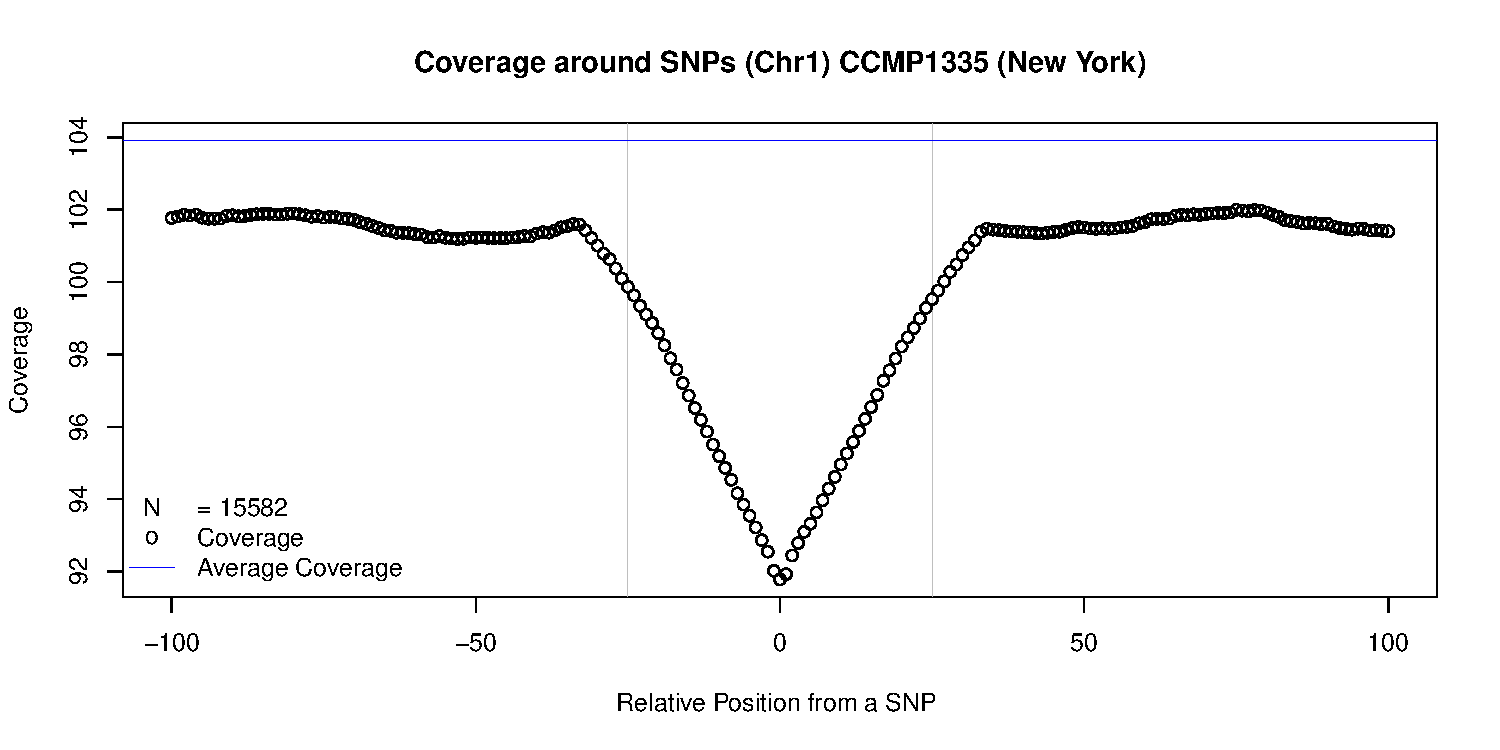
\includegraphics[width=\linewidth]{FigS5-SNPdip-figs/snpdip-chr1-1335.pdf}
\end{center}
\caption{{\bf Suggested Caption: Read depth near SNPS.} Plotted is the read depth within $\pm100$ nucleotides of single nucleotide polymorphisms (SNPs) identified by SAMtools, averaged over all 15582 SNPs called on Chromosome 1 of CCMP 1335.  X-axis: distance from SNP (bp).  Y-axis: read depth.  Horizontal blue line: average read depth across Chromosome 1.  Vertical grey lines: $\pm25$bp from SNP.  [[FOLLOWING TEXT IS PROBABLY BETTER IN THE ACCOMPANYING PROSE THAN IN THE CAPTION, BUT SOMEWHERE, SAY SOMETHING LIKE: CCMP1335 was sequenced with a mixture of 25bp mate-paired reads and 36bp single-end reads (TONY: ARE THESE NUMBERS CORRECT?).  The vertical grey lines in the figure mark the range in which the 25bp reads could simultaneously include the indicated position and the central SNP.  The probability that a randomly placed read covering a position $d$ base pairs away from the central SNP will \emph{not} cover the SNP rises linearly with $|d|$, which presumably explains the observed linear increase in coverage over the $\pm$read length interval.]]}
\end{figure}

Here are the others for comparison; pick whichever.

\noindent%
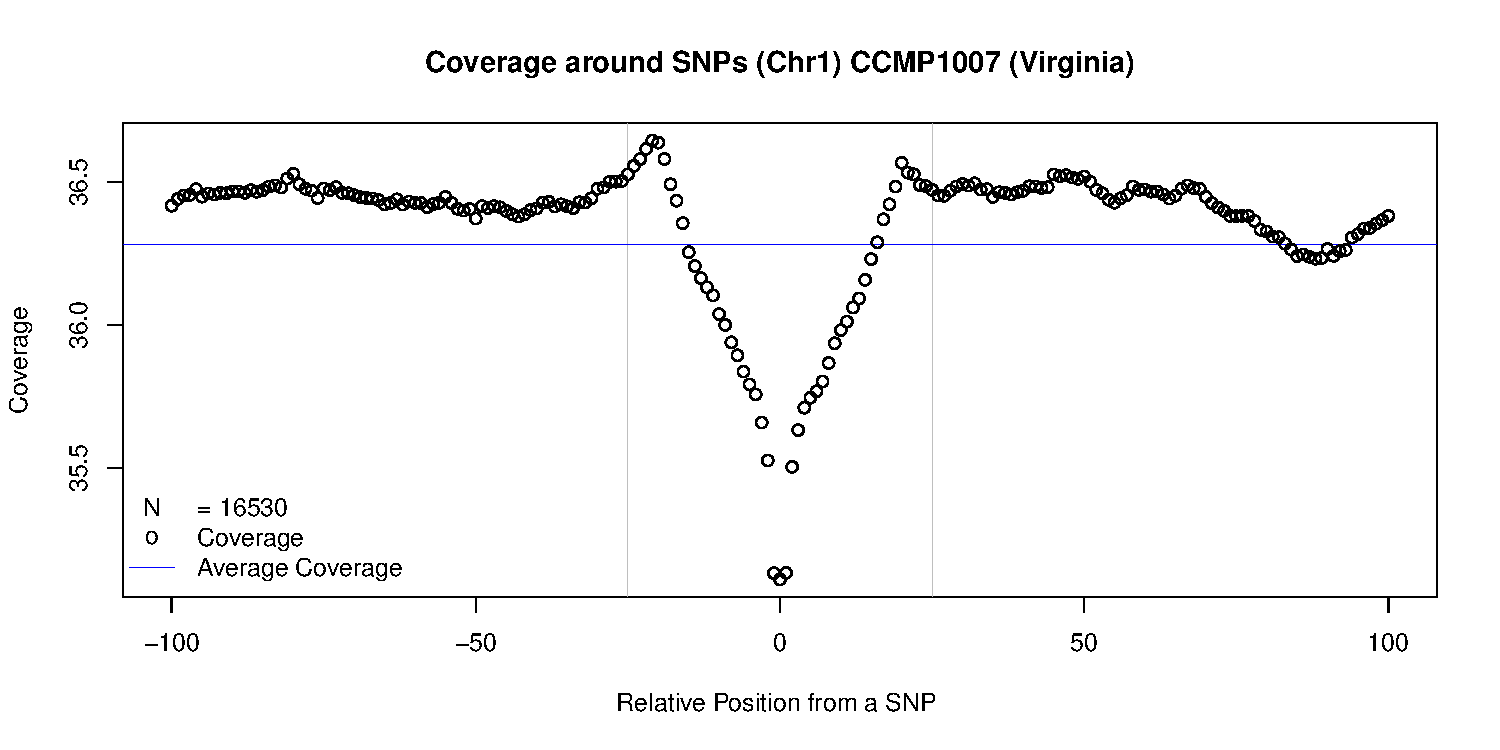
\includegraphics[width=\linewidth]{FigS5-SNPdip-figs/snpdip-chr1-1007.pdf}\\
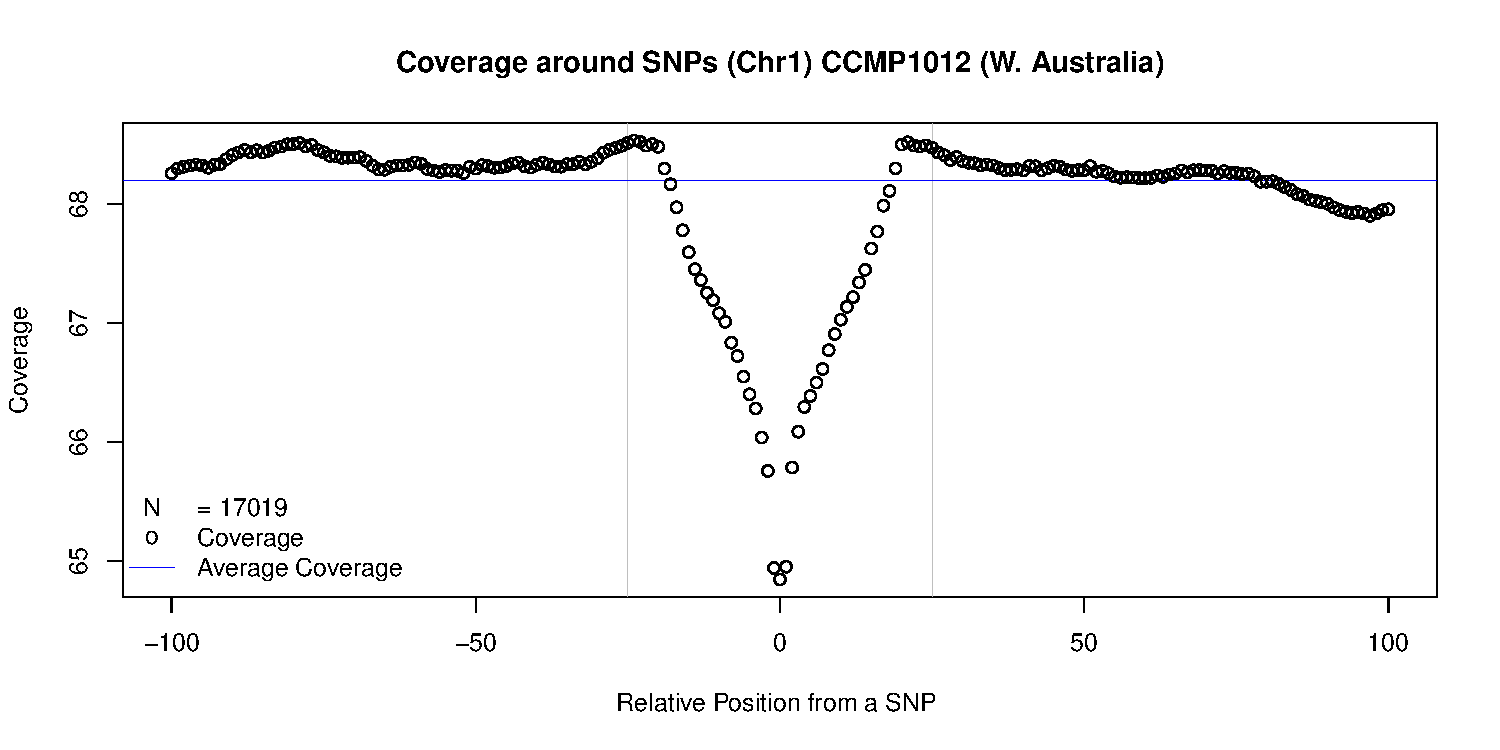
\includegraphics[width=\linewidth]{FigS5-SNPdip-figs/snpdip-chr1-1012.pdf}\\
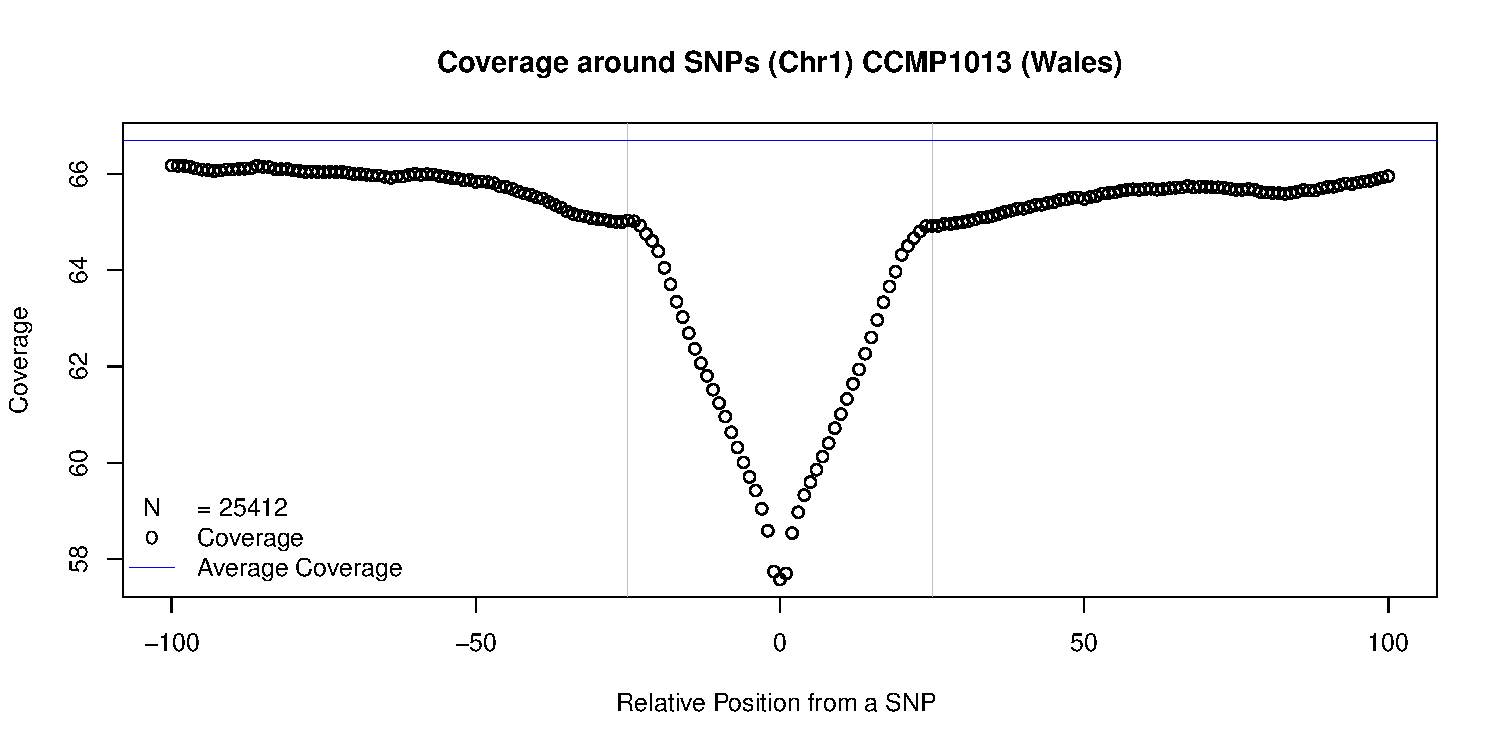
\includegraphics[width=\linewidth]{FigS5-SNPdip-figs/snpdip-chr1-1013.pdf}\\
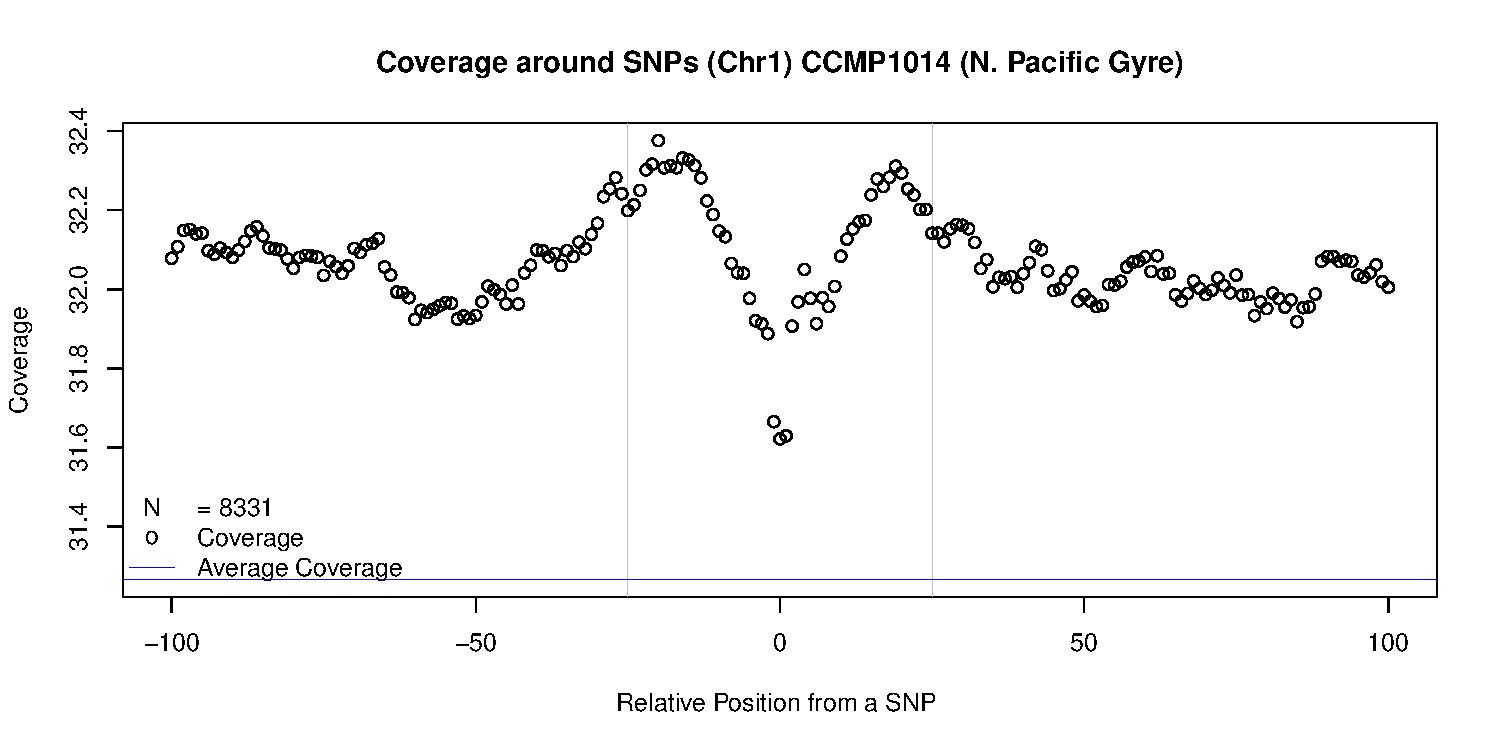
\includegraphics[width=\linewidth]{FigS5-SNPdip-figs/snpdip-chr1-1014.pdf}\\
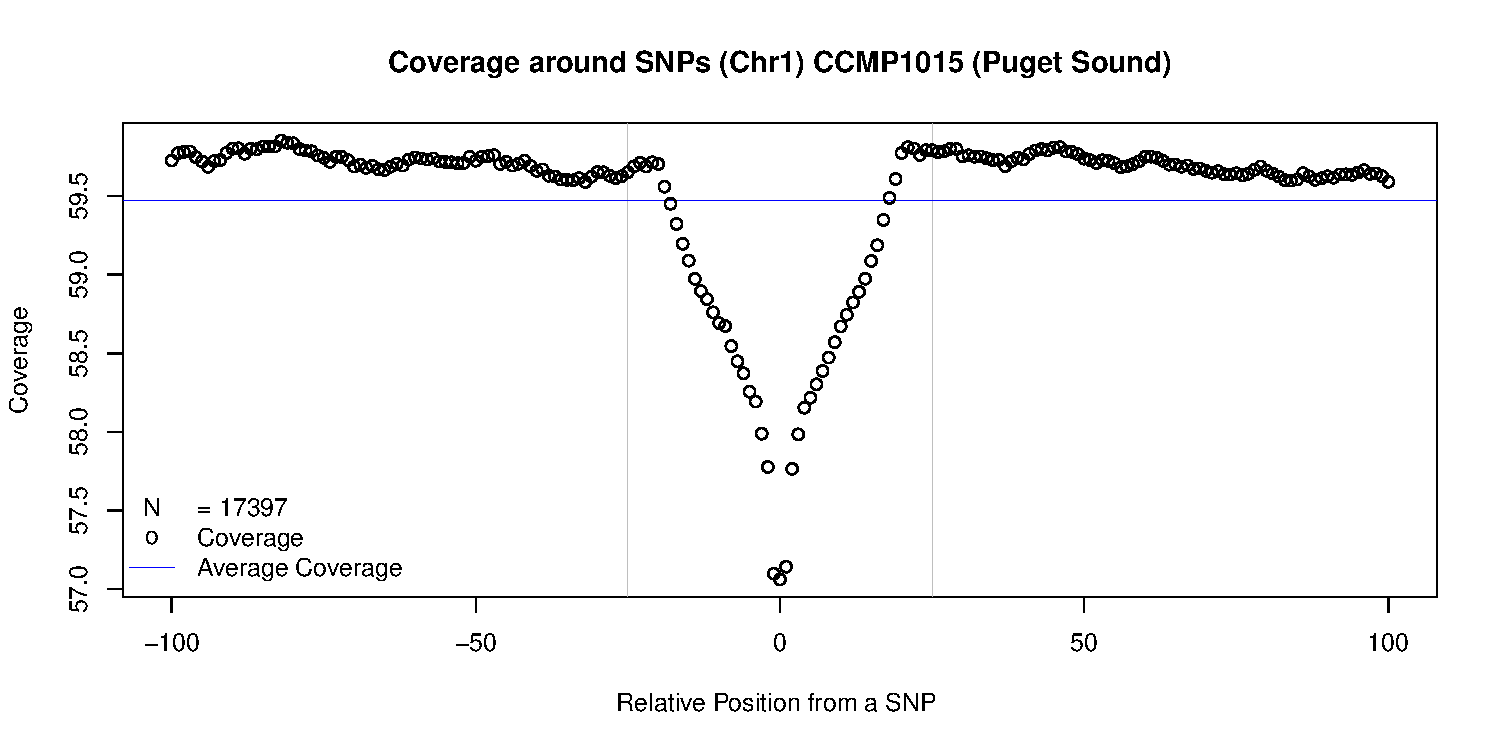
\includegraphics[width=\linewidth]{FigS5-SNPdip-figs/snpdip-chr1-1015.pdf}\\
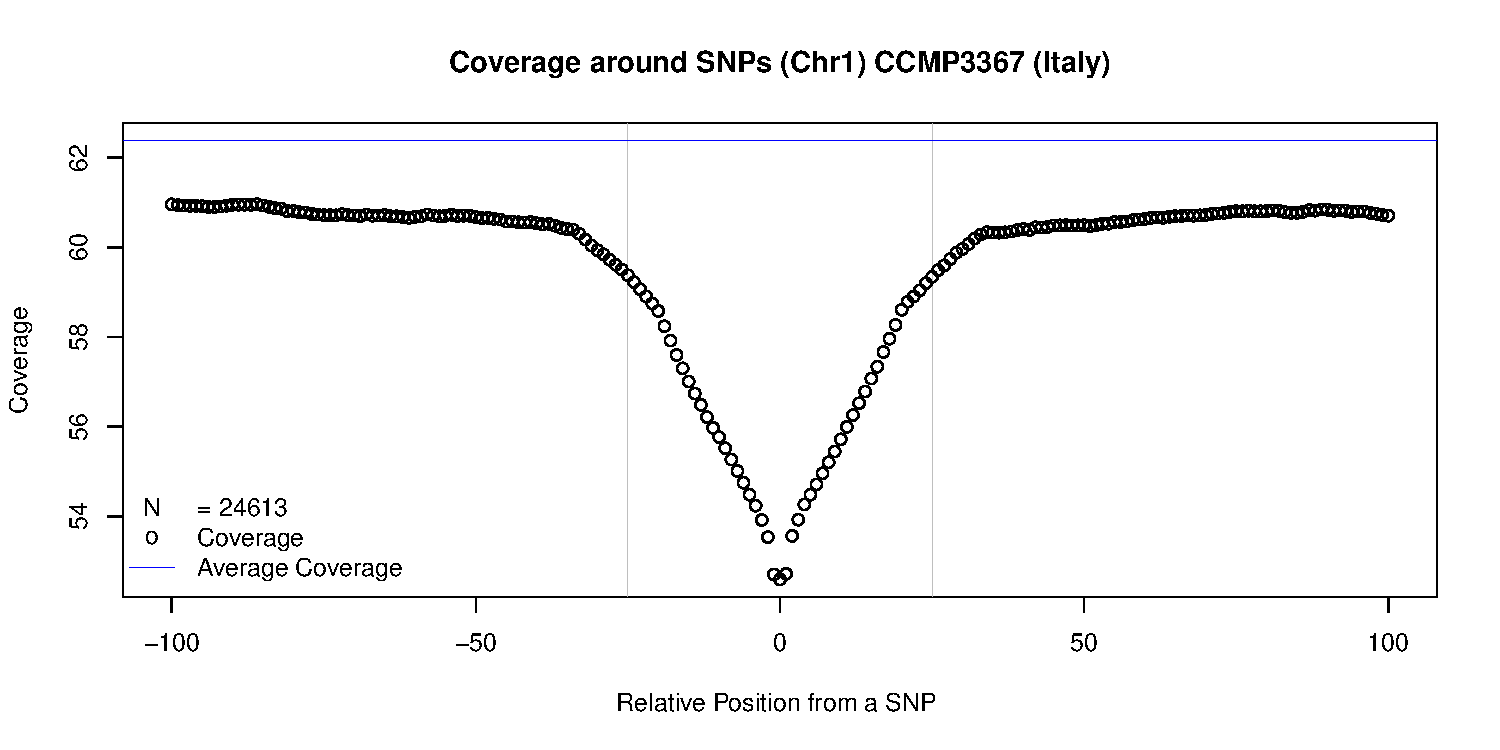
\includegraphics[width=\linewidth]{FigS5-SNPdip-figs/snpdip-chr1-3367.pdf}\\


% remember to do this to enable Id keyword substution: svn propset svn:keywords Id ed3.rnw 
\vfill\footnotesize\flushright SVN ID I miss you $ $Id: FigS5-SNPdip.rnw 2017-05-29 or later ruzzo $ $
\end{document}
